\chapter{Desenvolvimento do USP Kart}

No desenvolvimento do USP Kart, foram utilizadas diversas ferramentas e tecnologias para a implementação de um jogo de corrida estilo \textit{Kart} em 2.5D, com gráficos 3D e lógica bidimensional. Neste capítulo, serão apresentadas as principais ferramentas e tecnologias utilizadas, bem como a implementação de cada uma delas.

Primeiramente é necessário destacar que para que tudo fosse implementado foram necessários mais de uma categoria de padrão de projeto, como o \textit{Singleton}, por exemplo, este sendo o mais citado pelos gerenciadores e controladores de recursos, para serem acessados de qualquer lugar do código.

Também é importante destacar que o desenvolvimento do jogo foi feito em C++, utilizando de diversas bibliotecas e \textit{frameworks} para a implementação de cada parte do jogo, como o OpenGL para a renderização dos gráficos, o OpenAL para a reprodução de áudios, o Assimp para a importação de modelos 3D, entre outros.

Já que a linguagem C++ foi escolhida foi utilizado de paralelismo para a execução de várias tarefas, em destaque a separação da lógica do jogo e a renderização dos gráficos, para que o jogo possa ser o mais otimizado possível.

\section{Ferramentas desenvolvidas}

Como o jogo não possui um motor de jogo, foi necessário implementar diversas ferramentas e sistemas para ser desenvolvido. Dentre as principais estão o gerenciador de recursos, o gerenciador de configurações gráficas, o registrador de mensagens, o sistema gráfico e a classe de dados.

\subsection{Gerenciador de recursos}

O gerenciador de recursos foi implementado principalmente para garantir que todos os recursos fossem carregados e processados uma única vez, ou seja, um modelo em 3D de um kart não seria carregado mais de uma vez, evitando assim a duplicação de dados e economizando memória. Para isso, o gerenciador de recursos foi implementado com o padrão de projeto \textit{Singleton}, para que possa ser acessado de qualquer lugar do código e garantir que somente uma instância seja criada.

O funcionamento disso se dá através de um \textit{map} que armazena todos os recursos carregados, e ao requisitar um recurso, o gerenciador verifica se ele já foi carregado, e caso não tenha sido, ele é carregado e armazenado no \textit{map}.

\subsubsection{Texturas}

As texturas são um dos recursos carregados pelo gerenciador. Para implementar essa lógica foi criado uma classe \textit{Texture} que armazena o ID da textura, o caminho do arquivo, tipo da textura, tamanho, quantidade de canais e o dado bruto (utilizado somente pelo OpenGL).

\subsubsection{Ícones}

Também no gerenciador de recursos foi implementado o carregamento de ícones, apesar de não ser tão necessário, pois não é preciso carregar mais de uma vez, foi implementado para manter a consistência do código, uma vez tão semelhante ao carregamento de texturas.

Apesar da semelhança vale lembrar que os ícones são mais simples que texturas, é salvo somente seus dados brutos, mas mesmo assim, também para garantir uma boa organização, facilitando não só o armazenamento dos dados, mas a consistência entre diferentes plataformas. 

Já que o USP Kart foi desenvolvido em duas máquinas, uma com Windows e outra com Linux, foi necessário tratar diferentemente, principalmente por dificuldades com a lógica de ícones no \textit{Wayland}, servidor gráfico padrão do Linux.

\subsubsection{Modelos 3D}

Modelos no USP Kart foram importados utilizando a biblioteca Assimp, que é uma biblioteca de código aberto que permite a importação de modelos 3D de diversos formatos, como \textit{.obj}, \textit{.fbx}, \textit{.dae}, entre outros. No USP Kart, os modelos foram importados no formato \textit{.obj}, que é um formato simples e amplamente utilizado, além de que foi mais fácil de ser implementado uma vez que foi utilizado o programa \textit{Blockbench} para a modelagem dos personagens e karts.

Nessa classe de dados temos o que o Assimp chama comumente de \textit{mesh}, que é a malha do modelo, utilizado para renderizar o modelo, e o que o Assimp chama de \textit{material}, que é a textura do modelo, utilizado para renderizar a textura.

Como os modelos são bem mais pesados do que qualquer outro recurso, o sistema funciona de uma forma como \textit{cache}, ou seja, o modelo é carregado e armazenado na memória, e ao requisitar o modelo o sistema desempenha muito melhor do que se fosse carregar o arquivo toda vez que ele fosse requisitado.

\subsubsection{Áudios}

Os áudios são um dos recursos mais simples de serem carregados, visto que o OpenAL, biblioteca utilizada para a reprodução de áudios, já possui uma função que carrega o áudio e retorna um ID, usado para reproduzir o áudio. Dessa forma, o áudio é carregado e armazenado no \textit{map} do gerenciador, aonde retornamos o dado bruto.

\subsection{Gerenciador de configurações gráficas}\label{sec:gerenciador-de-configuracoes-graficas}

No desenvolvimento do USP Kart foram encontrados problemas gráficos e foi preciso implementar um gerenciador de configurações gráficas, para que o jogador possa ajustar as configurações gráficas do jogo, como resolução, modo de tela, posicionamento, entre outros.

As configurações são muito simples e armazenadas em um arquivo \textit{config.json} de configuração, não sendo acessível normalmente por uma interface gráfica, somente pelo arquivo em si e por meio de controles de janela, como redimensionar e mover, o que salva automaticamente as configurações.

O gerenciador também é um \textit{Singleton}, para garantir que somente uma instância seja criada e que as configurações sejam as mesmas em todo o jogo, além disso, caso o programa quebre por qualquer motivo que seja temos um controlador que garante que mesmo assim as configurações sejam salvas.

\subsection{Registrador de mensagens}

É muito comum em motores de jogo terem um sistema de mensagens, muito útil para depurar o código e encontrar possíveis erros. No USP Kart foi implementado um sistema de mensagens, com níveis de importância, para que o desenvolvedor possa encontrar possíveis erros no código, aonde o sistema de mensagens é um \textit{Singleton}.

Cada mensagem contém um registro da hora em que a mensagem foi enviada, um nível de importância, o arquivo e linha onde foi chamada, além do texto. O sistema de mensagens é muito simples, mas muito eficaz, e implementado para que o desenvolvedor possa encontrar possíveis erros no código, sem a necessidade de depurar o código.

\subsubsection{Fila}

Como o jogo tem muitos elementos assíncronos, foi necessário implementar uma fila de mensagens, para que as mensagens sejam processadas de forma assíncrona, aguardando a próxima ser processada, evitando que a sua escrita seja interrompida por outra.

Isso foi implementado usando o que é chamado \textit{mutex}, um mecanismo de sincronização que permite que somente uma \textit{thread} possa acessar um recurso por vez, garantindo que a fila de mensagens seja processada corretamente.

\subsubsection{Escrita em arquivo}

Como no sistema era bem comum que problemas no desenvolvimento fossem encontrados, matando o processo do jogo e dificultando a depuração. Para isso, foi implementado um sistema de escrita em arquivo, para que as mensagens fossem salvas em um arquivo padronizado por data, como '\textit{\{ano\}\{mês\}\{dia\}.log}' (por exemplo: \textit{20241201.log} para o dia 01/12/2024).

Dessa forma, caso ocorra um erro fatal, responsável por matar o processo, as mensagens são salvas em um arquivo, permitindo que o desenvolvedor possa encontrar o erro e corrigi-lo.

\subsection{Sistema de interface gráfica}

A interface gráfica do jogo foi o mais simples o possível, por dificuldades técnicas, mas também por escolha do desenvolvedor de usar a biblioteca ImGUI. Ela é composta por um texto no canto superior esquerdo da tela, que mostra a posição do jogador e a quantidade de quadros por segundo sendo desenhados, e um texto no canto superior direito da tela, que mostra a quantidade de voltas completadas.

O sistema de interface gráfica é um \textit{Singleton}, como vários outros sistemas, para garantir que somente uma instância seja criada e gerenciada de forma correta. A interface gráfica é muito simples, mas muito eficaz, e implementada para que o jogador possa acompanhar a corrida e a quantidade de voltas completadas.

\subsubsection{Fila}
Como o registrador de mensagens, o sistema de interface gráfica também possui uma fila, para que os componentes a serem desenhados sejam processados de qualquer lugar, e, ao final da renderização da tela pelo OpenGL, limpamos toda a fila, garantindo que todos os componentes requeridos durante a lógica do jogo sejam desenhados.

\subsubsection{Texto}

O componente principal desenhado pela interface gráfica é o texto, composto de um texto, tamanho da fonte, cor, posição e borda (com sua respectiva cor escolhida também), e desenhado utilizando o OpenGL e a biblioteca ImGUI, carregando uma fonte livre externa, para que o componente seja processado corretamente.

\subsection{Classe de dados}

A classe de dados não é um \textit{Singleton} como os outros componentes do jogo, justamente porque é completamente mutável, utilizada para armazenar dados utilizados em todo o jogo, como os objetos processados e até mesmo com a inicialização da lógica dos personagens.

Ela foi implementada mais por organização, já que o jogo é muito complexo e possui muitos elementos mutáveis, e a classe de dados foi implementada para que todos os dados sejam armazenados em um único lugar, facilitando a organização e a manutenção do código.

\section{Gráficos com OpenGL}

Toda a parte gráfica do jogo foi feita utilizando o OpenGL, uma API de baixo nível para renderização de gráficos 2D e 3D, que permite a criação de gráficos de alta qualidade e desempenho. O OpenGL foi escolhido por ser uma biblioteca amplamente utilizada e bem documentada, além de ser compatível com várias plataformas, como Windows, macOS e Linux.

Também foi necessário utilizar o GLEW, uma biblioteca que facilita o uso de extensões do OpenGL, o GLFW, uma biblioteca que facilita a criação de janelas e o gerenciamento de eventos, para a criação da janela do jogo e o gerenciamento de eventos de teclado e mouse e o GLM, que manipula matrizes e vetores, para calcular as transformações dos objetos.

Vale a pena lembrar que todas as bibliotecas utilizadas são de código aberto multiplataforma, garantindo que o jogo seja compatível com diferentes sistemas operacionais, como foi necessário para o desenvolvimento do USP Kart.

\subsection{Criação de janela}

Para criar janelas o GLFW foi utilizado, nele é possível criar janelas, gerenciar eventos de teclado e mouse, e  contextos OpenGL. A janela tem opções de configuração, todas elas são configuradas no gerenciador de configurações gráficas \ref{sec:gerenciador-de-configuracoes-graficas}, como resolução, modo de tela, posicionamento, entre outros.

\subsection{Gerenciador de controles}\label{sec:gerenciador-de-controles}

Para gerenciar os controles foi criado um sistema para isso, um \textit{Singleton} responsável por armazenar funções a serem executadas quando uma tecla é pressionada, funciona por um sistema de filas que, ao pressionar uma tecla, executa todas as funções armazenadas na fila associadas aquele botão.

\subsection{Shaders}

Os \textit{shaders} são programas escritos em GLSL, uma linguagem de programação de alto nível para shaders, executados na GPU e controlam a renderização dos gráficos. No USP Kart, foram utilizados dois \textit{shaders}, um para a renderização dos objetos e outro para depuração das caixas de colisão.

Para implementar uma lógica mais alto nível para a manipulação dos \textit{shaders}, foi criado uma classe de mesmo nome, responsável por carregar, compilar e passar variáveis para os \textit{shaders}, facilitando a implementação e a manutenção dos \textit{shaders}.

\subsection{Texturas}

As texturas também são gerenciados pelo OpenGL, mas para facilitar a manipulação das texturas, foi criado uma classe \textit{Texture}, que armazena dados como ID da textura, caminho do arquivo, tipo da textura, tamanho, quantidade de canais e o dado bruto (utilizado somente pelo OpenGL).

O gerenciador de recursos é responsável por carregar e armazenar as texturas, como falado anteriormente, e a classe \textit{Texture} é responsável por manipular as texturas, como carregar, descarregar e renderizar. Ela é principalmente utilizado pelos modelos 3D, que têm texturas associadas ao mesmo.


\subsection{Modelos 3D}

Os modelos 3D são importados utilizando a biblioteca Assimp, que é uma biblioteca de código aberto que permite a importação de modelos 3D de diversos formatos, como \textit{.obj}, \textit{.fbx}, \textit{.dae}, entre outros. No USP Kart, os modelos foram importados no formato \textit{.obj}, que é um formato simples e amplamente utilizado, além de que foi mais fácil de ser implementado uma vez que foi utilizado o programa \textit{Blockbench} para a modelagem dos personagens e karts.

Os modelos 3D são compostos por \textit{meshes}, que são as malhas do modelo, e \textit{materials}, são as texturas do modelo. Para renderizar os modelos 3D, é necessário passar as malhas e texturas para o OpenGL, responsável renderizar os modelos na tela.

Toda a lógica foi pensada em como o Assimp gerencia os modelos, e como o OpenGL renderiza os modelos, para que a implementação seja o mais otimizada possível, e o jogo seja o mais rápido e dinâmico possível.

\subsection{Skybox}

O \textit{Skybox} é uma técnica utilizada para simular um céu em jogos 3D, composto por seis texturas, uma para cada face de um cubo, que são renderizadas ao redor do jogador, criando a ilusão de um céu infinito. No USP Kart, o \textit{Skybox} foi implementado utilizando seis texturas de um céu azul, renderizadas ao redor do jogador, criando a ilusão de um céu infinito.

Existem outras formas de se implementar um \textit{Skybox}, como utilizando um cilindro ou uma esfera, mas no USP Kart foi utilizado um cubo, por ser mais simples e mais fácil de implementar, e por ser mais eficiente em desempenho.

\subsection{Animação}

Basicamente os objetos são todos estáticos, mas eles podem ter outros modelos associados aonde são animados para condizer com a lógica programada, como a animação de movimentação dos karts, elaborado para animar a rotação das rodas ao esterçar.

\section{Mapa}

O mapa foi feito da maneira o mais simples o possível, com um objeto de quatro vértices, fazendo assim um plano quadrado de 256x256 unidades de tamanho, colocado no plano XZ, foi pego uma textura do mapa \textit{Donut Plains 1} do \textit{Mario Kart} (\cite{marioKart}), e aplicado no objeto.

\subsection{Modelagem do mapa}

Para que o mapa fosse utilizável foi necessário traduzi-lo para uma imagem em tons de cinza, onde quanto mais escuro o ponto, mais fácil é de se passar por ele, e quanto mais claro, mais difícil. O mapa foi modelado para que o jogador não possa passar por pontos (totalmente) brancos, e que a estrada, totalmente preta, seja a forma preferível de se passar.
\subsection{Pontos de controle}

Também conhecido como 'ponto de checagem', o ponto de controle serve para verificar se o jogador está no caminho correto, ou seja, esteja progredindo e se aproximando da linha de chegada. No USP Kart, os pontos de controle são invisíveis ao jogador, mas a lógica de todos os personagens (controlados pelo jogador ou não) conhecem e baseam-se neles para saber sua posição relativa ao mapa.

\subsection{Controlador do mapa}

Para gerenciar tudo o que é relacionado ao mapa, foi elaborado um controlador, onde sua responsabilidade é traduzir coordenadas do mundo para coordenadas do mapa, e vice-versa, além de verificar se um ponto está no mapa, e buscar caminhos de um ponto a um ponto de controle (em inglês, \textit{checkpoint}).

O que os personagens (em inglês, \textit{characters}) pedem para o controlador é mostrar qual o caminho mais próximo para o próximo ponto de controle, e o mesmo retorna o caminho, uma lista de pontos, que o personagem deve seguir para chegar ao ponto de controle.

Uma representação visual do que o personagem deve seguir pode ser desenhado pelo programa, segue o exemplo:

\begin{figure}[H]
    \centering
    \begin{subfigure}[t]{0.45\textwidth}
        \centering
        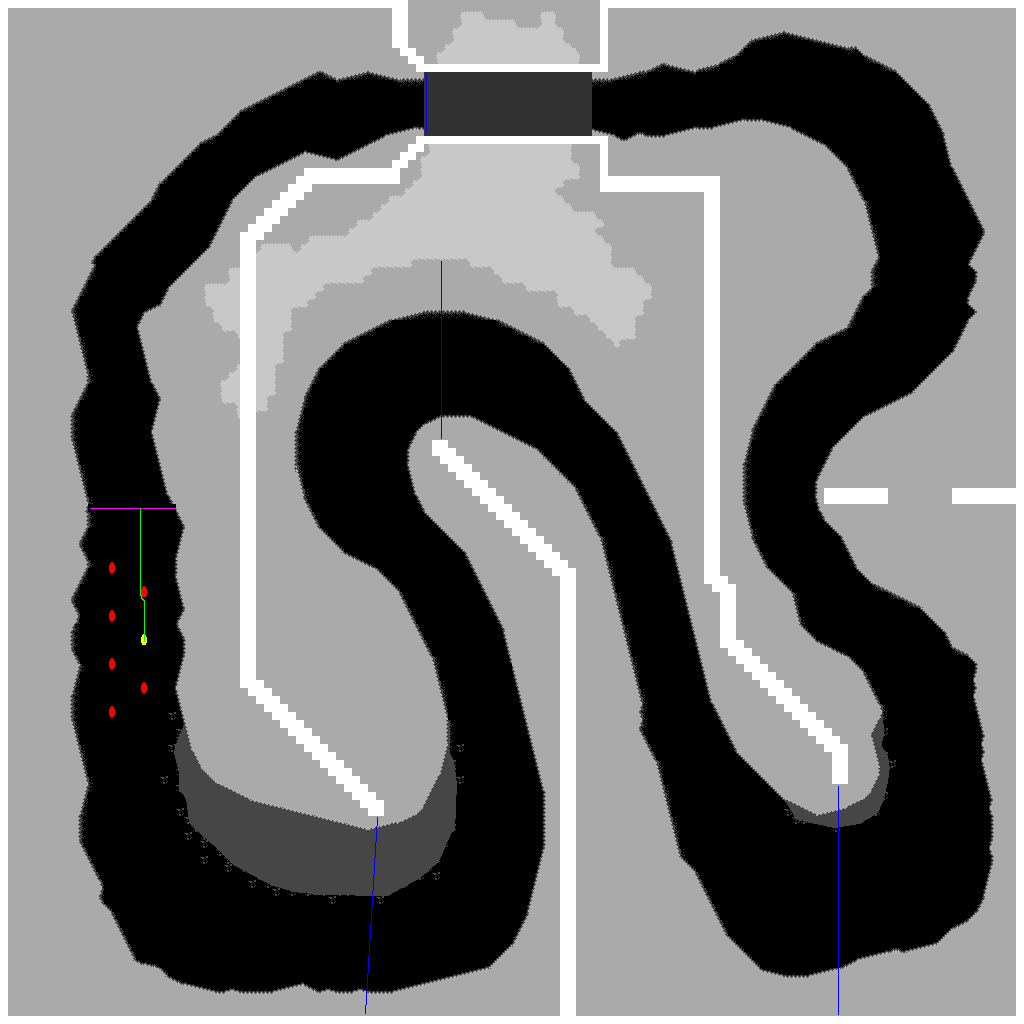
\includegraphics[width=0.8\textwidth]{figuras/Mapa modelado.png}
        \caption{Imagem impressa pelo controlador do mapa no USP Kart.}
        \label{fig:mapa-modelado}
    \end{subfigure}
    \hfill
    \begin{subfigure}[t]{0.45\textwidth}
        \centering
        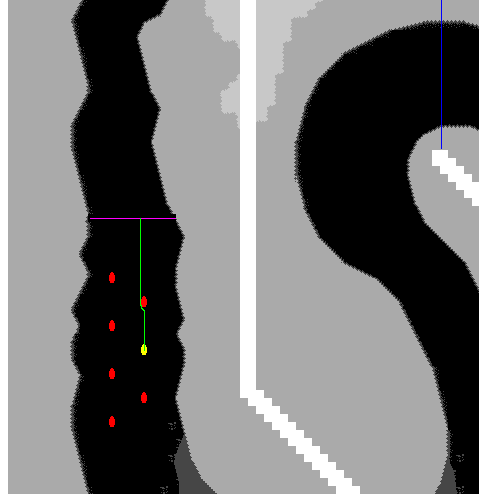
\includegraphics[width=0.8\textwidth]{figuras/Mapa modelado cortado.png}
        \caption{Corte da imagem para melhor visualização}
        \label{fig:mapa-modelado-com-pontos}
    \end{subfigure}
    \caption{Mapa do USP Kart.}
    \footnotesize{A figura à esquerda \textbf{(a)} mostra o mapa modelado utilizado no jogo, enquanto a figura à direita \textbf{(b)} destaca a estrada em preto e as paredes intransponíveis em branco, além de pontos coloridos, como o amarelo, que representa o observador (ponto de início do cálculo do caminho), os pontos vermelhos (objetos colidíveis), os pontos azuis (pontos de controle), os pontos verdes (caminho mais curto a ser seguido) e os pontos roxos (próximo ponto de controle)}
    \label{fig:mapa-usp-kart}
\end{figure}

\section{Lógica por objetos}

A lógica do jogo funciona por objetos, cada um contém um modelo associado, além de informações como posição, rotação, escala, velocidade, aceleração, entre outros. A lógica é dividida em dois tipos de objetos, os objetos estáticos e com física.

Com a lógica por objetos, é possível implementar a física do jogo, como a movimentação dos karts, a colisão com objetos e outros personagens, a detecção de colisão, a resolução de colisão, entre outros.

Tudo o que aparece na tela é um objeto, e existem vários tipos que estendem essa classe, como os personagens, os karts, os objetos estáticos, os objetos com física, entre outros.

\subsection{Modelos de objetos}

Os modelos dos objetos são totalmente coletados pela biblioteca Assimp, e são armazenados no gerenciador de recursos, cada objeto tem um endereço que aponta para o modelo, dessa forma, vários objetos podem ter o mesmo modelo, mas com posições, rotações e escalas diferentes, facilitando assim, o carregamento na placa de vídeo pelo OpenGL.
\subsection{Transformações}

O OpenGL trabalha com matrizes, e para que um objeto seja renderizado na tela, é necessário passar as transformações do objeto para o OpenGL, como a posição, rotação e escala. Para isso, foi criado uma função para calcular uma matriz de transformação do modelo, passada para o \textit{shader} de renderização.

\begin{programruledcaption}{Código de cálculo da matriz de transformação do modelo.).\label{prog:model}}
    \begin{lstlisting}[
      language={C++},
      style=wider,
      functions={},
      specialidentifiers={},
    ]
    glm::mat4 getModel(const glm::mat4 &baseModel) const
{
    auto m_model = baseModel;
    m_model = translate(m_model, pos);
    m_model = glm::scale(m_model, glm::vec3(scale.x, scale.y, scale.z));
    m_model = glm::rotate(m_model, angle.x, glm::vec3{1, 0, 0});
    m_model = glm::rotate(m_model, angle.y, glm::vec3{0, 1, 0});
    m_model = glm::rotate(m_model, angle.z, glm::vec3{0, 0, 1});
    return m_model;
}
    \end{lstlisting}
\end{programruledcaption}

\section{Modelagem dos karts}

Para a representação visual dos karts foi utilizado um modelo do kart propriamente dito sem as rodas, e separadamente outro modelo somente das rodas, já que a animação do jogo procedural é feita pela lógica do jogo, e não pela animação do modelo.

\subsection{Bicycle model}

Para essa representação visual foi utilizado do modelo \textit{bicycle model}, representação que considera a separação do carro (ou no caso, kart) em duas rodas, a dianteira e a traseira.

O modelo de bicicleta (em inglês, \textit{Bicycle Model}) é amplamente utilizado em aplicações de dinâmica veicular, computação gráfica e inteligência artificial. Trata-se de uma representação simplificada, porém eficaz, da cinemática e dinâmica de veículos terrestres. Seu nome é 'modelo de bicicleta' porque reduz o comportamento de um veículo de quatro rodas a um sistema de duas rodas em linha, eliminando a necessidade de modelar individualmente cada roda.

\subsubsection{Princípios Fundamentais}

O modelo de bicicleta opera sob o princípio de que as rodas dianteira e traseira representam os eixos de direção e tração do veículo, respectivamente. Ele captura o movimento veicular utilizando parâmetros como ângulo de esterçamento, velocidade, aceleração, e forças de tração. Embora simplificado, o modelo mantém precisão suficiente para aplicações como simulação de trajetória e controle autônomo em veículos.

\subsubsection{Vantagens e Limitações}

A simplificação do modelo reduz a complexidade computacional, ideal para uso em simulações em tempo real. Ele é especialmente eficaz em cenários de baixa velocidade e onde o deslizamento das rodas não é significativo. No entanto, suas limitações incluem a dificuldade em capturar dinâmicas mais complexas, como derrapagens ou comportamentos em altas velocidades, que requerem modelagens dinâmicas mais avançadas, como o modelo de veículo completo (\textit{Full Vehicle Model}).

\begin{figure}[H]
    \centering
    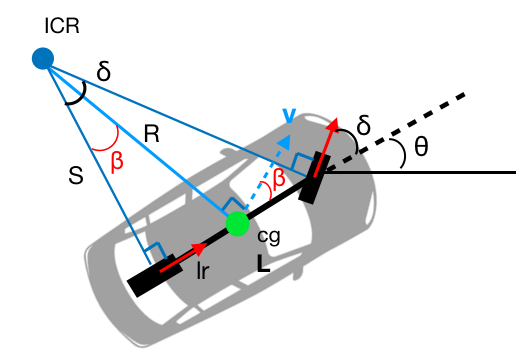
\includegraphics[width=0.8\textwidth]{figuras/Bicycle Model.png}
    \caption{Modelo de bicicleta (\textit{Bicycle Model}).}
    \footnotesize{Fonte da imagem: \cite{bicycleModel}}
    \label{fig:bicycle-model}
\end{figure}
\pagebreak

\begin{programruledcaption}{Código de atualização do modelo de bicicleta (\textit{Bicycle Model}).\label{prog:bicycle}}
    \begin{lstlisting}[
      language={C++},
      style=wider,
      functions={},
      specialidentifiers={},
    ]
    void updateBicycleModel(const float deltaTime)
    {
        const auto speed = getSpeed();
        if (speed == 0)
            return;
    
        // 'this->angle' = omega
        // 'this->steeringAngle' = delta
        // 'this->speed' = v
    
        const auto frontWheel = (frontWheels[0].getPos() + frontWheels[1].getPos()) * 0.5f;
        const auto backWheel = (backWheels[0].getPos() + backWheels[1].getPos()) * 0.5f;
        const auto L = glm::distance(glm::vec3(frontWheel), glm::vec3(backWheel));
    
        // Calculate the new angle of the kart based on the current speed and steering angle
        float angularSpeed = speed / L * std::tan(steeringAngle);
        const auto angleChange = angularSpeed * deltaTime;
    
        // Update the angle of the kart
        angle.y += angleChange;
    
        velocity = forward() * getSpeed();
    }
    \end{lstlisting}
\end{programruledcaption}

\subsection{Implementação das rodas}

As rodas do carro foram implementadas separando em traseiras e dianteiras, sendo as dianteiras responsáveis pela direção e as traseiras pela tração, e a animação das rodas foi feita pela lógica do jogo, e não pela animação do modelo.

Pelo modelo de bicicleta, as rodas dianteiras são rotacionadas pelo ângulo de esterçamento, além de ambas (dianteiras e traseiras) são afetadas pela velocidade.

\section{Física}

Para implementar a física do jogo foi necessário adicionar uma quantidade de massa e tamanho para cada elemento, e a cada iteração do cálculo de jogo (ou \textit{frame}), a força é aplicada ao objeto, a aceleração é calculada, a velocidade é atualizada e finalmente a posição é atualizada.

\subsection{Objetos estáticos}

Esses objetos não têm massa, são os objetos padrões do jogo, não se pode fazer alteração nenhuma a eles, já que seus métodos de movimentação são vazios, sendo necessário sobrescrevê-los para que alguma ação seja efetuada, dessa forma, não é preciso fazer muitas checagens ao interagir com a física do jogo, economizando tempo e memória.

\begin{programruledcaption}{Métodos da classe \textit{Object} vazios para objetos estáticos.\label{prog:mdc}}
    \begin{lstlisting}[
      language={C++},
      style=wider,
      functions={},
      specialidentifiers={},
    ]
      virtual void resolveCollisionWithLimits() {}
      virtual void applyCorrectionForce(const glm::vec3 &correctionForce, float massRatio) {}
      virtual glm::vec3 getAngularVelocity() const { return {0, 0, 0}; }
      virtual glm::vec3 *getAcceleration() { return nullptr; }
      virtual glm::vec3 *getVelocity() { return nullptr; }
      virtual void adjustPitch(const float value) {}
      virtual void treatCollision(Object &other) {}
      virtual void move(const glm::vec3 &value) {}
      virtual void resize(const float value) {}
      virtual void rotate(const float value) {}
      virtual float getInertia() const { return 0; }
      virtual float getMass() const { return 0; }
      virtual void init() {}
    \end{lstlisting}
\end{programruledcaption}

\subsection{Objetos com física}

Esses objetos são uma extensão dos objetos estáticos, mas com a adição de massa, inércia e aceleração, além de que a cada iteração do cálculo de jogo, a força é aplicada ao objeto, a aceleração é calculada, a velocidade é atualizada e finalmente a posição é atualizada.

Para implementar isso foi utilizado uma quantidade mínima de código, simplesmente sobrescrevendo os métodos da classe \textit{Object} (mostrados em \ref{code:object-methods}) e adicionando a lógica de física, como a aplicação de força, cálculo de aceleração, atualização de velocidade e posição, entre outros.

\subsection{Movimentação}

A movimentação dos objetos devem ser feitos diretamente (auto-impulsionada, no caso dos karts) ou pela colisão com outros objetos, e a movimentação é feita pela aplicação de força, cálculo de aceleração, atualização de velocidade e posição, entre outros.

\subsubsection{Força}

A força é aplicada ao objeto pela lógica do jogo, afeta-o por um quadro calculado (não é salva pelo objeto), e é calculada pela fórmula $F = m \cdot a$, onde $F$ é a força, $m$ é a massa e $a$ é a aceleração.

Esse cálculo é feito a cada iteração do cálculo de jogo, e a força é aplicada ao objeto, afetando a aceleração e descartando a força, para que não seja aplicada novamente.

\subsubsection{Aceleração}

A aceleração é mantida no objeto, e é calculada pela fórmula $a = F / m$, onde $a$ é a aceleração, $F$ é a força e $m$ é a massa. Com essa fórmula, a aceleração é calculada a cada iteração do cálculo de jogo, e a velocidade é atualizada.

Depois de calculado a nova velocidade do objeto, calculamos uma aceleração constante com direção contrária a velocidade, para que o objeto pare de se mover caso não haja mais força sendo aplicada, sendo assim considerado o atrito.

\subsection{Colisão}

Para o tratamento de colisão foi implementado uma caixa de colisão (em inglês, \textit{collision box}) para cada objeto, sendo uma elipsoide para a lógica em duas dimensões (2D) do jogo, e a colisão é detectada pela interseção das caixas de colisão dos objetos.

\begin{figure}[H]
    \centering
    \includegraphics[width=0.8\textwidth]{figuras/Caixa de Colisão.png}
    \caption{Caixa de colisão dos objetos.}
    \footnotesize{A figura mostra a caixa de colisão como uma elipsoide (estendida no eixo y para melhor visualização, assim apresentando-se como um cilindro)}
    \label{fig:collision-box}
\end{figure}

\subsubsection{Detecção de colisão}

Para a detecção de colisão foi implementado um sistema de caixas de colisão, que são caixas que envolvem o objeto, e a colisão é detectada pela interseção das caixas de colisão dos objetos, e a detecção é feita a cada iteração do cálculo de jogo.

O algoritmo de detecção é o mais simples o possível, detectando as linhas projetadas em 2D que se interceptam e a detecção é feita a cada iteração do cálculo de jogo. O nome do algoritmo é \textit{Separating Axis Theorem} (SAT), e é amplamente utilizado em jogos 2D.

O teorema SAT, como descrito em \cite{SAT:separatingAxisTheorem}, afirma que dois objetos convexos são disjuntos se existir ao menos um eixo em que as projeções dos dois objetos não se sobreponham. A abordagem consiste em identificar e testar os eixos de separação potenciais, que são definidos pelas normais das faces dos polígonos ou pelos produtos vetoriais entre as arestas dos objetos. Para cada eixo identificado, calculam-se as projeções dos vértices dos objetos e verifica-se se as projeções apresentam interseção. Se não houver sobreposição em pelo menos um eixo, os objetos não colidem.

\begin{figure}[H]
    \centering
    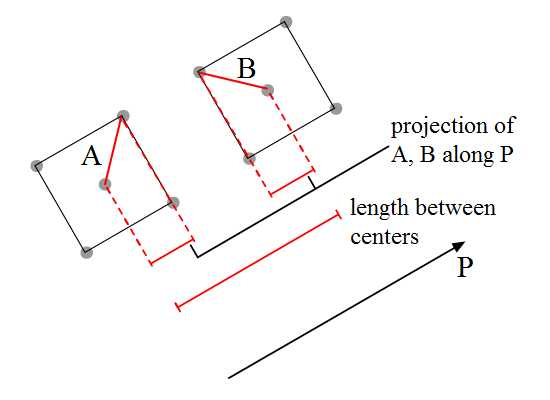
\includegraphics[width=0.8\textwidth]{figuras/SAT.jpg}
    \caption{Imagem exemplo de detecção de colisão com o \textit{Separating Axis Theorem} (SAT).}
    \footnotesize{Fonte da imagem: \cite{SAT:separatingAxisTheorem}}
    \label{fig:sat_example}
\end{figure}

O código aplicado retorna uma estrutura que chamamos de \textit{CollisionData}, composto da penetração, a normal da colisão e o ponto de colisão, para que a resolução de colisão seja feita.

\pagebreak
\begin{programruledcaption}{Código de detecção de colisão}
    \begin{lstlisting}[
        language={C++},
        style=wider,
        functions={},
        specialidentifiers={},
    ]
    CollisionData CollisionBox::getCollisionForce(const CollisionBox &other) const
    {
        const auto vertices1 = get2DProjectedVertices();
        const auto vertices2 = other.get2DProjectedVertices();

        for (size_t i = 0; i < vertices1.size(); i += 2)
        {
            const auto p1 = vertices1[i];
            const auto p2 = vertices1[(i + 2) % vertices1.size()];

            for (size_t j = 0; j < vertices2.size(); j += 2)
            {
                const auto q1 = vertices2[j];
                const auto q2 = vertices2[(j + 2) % vertices2.size()];

                glm::vec3 intersection;
                if (linesIntersect(p1, p2, q1, q2, intersection))
                {
                    glm::vec3 normal = glm::normalize(glm::vec3{p2.y - p1.y, 0, p1.x - p2.x});
                    return {glm::length(p2 - p1), normal, intersection};
                }
            }
        }

        return {0, {}, {}};
    }
    \end{lstlisting}
\end{programruledcaption}


\subsubsection{Resolução de colisão}

Para a resolução de colisão foi implementado um sistema de resolução de colisão, que é feito pela aplicação de uma força contrária à colisão, e a resolução é feita a cada iteração do cálculo de jogo.

O algoritmo de resolução é o mais simples o possível, aplicando uma força contrária à colisão, e a resolução é feita a cada iteração do cálculo de jogo.

\section{Personagens}

Os personagens (em inglês, \textit{characters}) são os jogadores e personagens não jogáveis (em inglês, \textit{non-playable characters} ou NPCs) do jogo, e são controlados pela lógica do jogo, e a lógica é dividida em dois tipos de personagens, os personagens controlados pelo jogador e os personagens controlados pela inteligência artificial.

Eles funcionam por meio de estados, pelo padrão de projeto \textit{State}, e a cada iteração do cálculo de jogo ele reage de acordo.

\subsection{Estados}

Ele tem três tipos de estados, o estado de esterço, estado de aceleração e estado de frenagem. Cada estado é responsável por uma ação, e a cada iteração do cálculo de jogo ele reage de acordo, por exemplo, caso o estado de aceleração esteja ativado a cada iteração o personagem recebe uma força que o acelera de acordo.

\subsection{Jogador}

O jogador é uma extensão do personagem, mas com a adição de controles por teclado. Ele é controlado pelo jogador, e a cada iteração do cálculo de jogo ele reage de acordo com os controles do jogador, e a lógica é dividida em dois tipos de jogadores, o jogador controlado pelo teclado e o jogador controlado pelo controle.

Na construção de sua classe é determinado as teclas utilizadas para cada ação, nele temos o que determinamos como 'lógica de mudança de estado', por exemplo, se o jogador pressionar a tecla de aceleração, o fator de estado de aceleração é ativado, e o personagem muda de estado.

\subsubsection{Controles}

Para mudar o estado do jogador foi utilizado o gerenciador de controles (ver: \ref{sec:gerenciador-de-controles}), que é um \textit{Singleton} responsável por armazenar funções a serem executadas quando uma tecla é pressionada, funciona por um sistema de filas que, ao pressionar uma tecla, executa todas as funções armazenadas na fila associadas aquele botão.

No caso do jogador ele tem uma espécie de função de chamada (em inglês, \textit{callback}), que é chamada quando a tecla é pressionada, e somente nesse momento, economizando em recursos para não precisar fazer uma checagem constante.

As teclas utilizadas foram as mais padrões, as setas direcionais para direção, aceleração e frenagem, para dar uma experiência mais simples.

\subsection{Inteligência artificial}

Também é uma extensão do personagem, mas com a adição de uma lógica de própria. Esse corredor é utiliza dos mesmos dados (de caminho e pontuação) que consegue da busca do caminho mais curto para o próximo ponto de controle.

Com mais uma \textit{thread} separada para a lógica de mudança de estado do personagem não jogável, ele consegue se movimentar de forma autônoma, sem a necessidade de interação do jogador.

\subsubsection{Visão ambiental}

Como todo corredor, ele chama o controlador do mapa para saber qual o caminho mais curto para o próximo ponto de controle, e com isso ele consegue ter uma visão do ambiente. A imagem mais clara sobre o que o corredor enxerga é a imagem \ref{fig:mapa-modelado-com-pontos}.

\subsubsection{Tomada de decisão}

Para a tomada de decisão o personagem não jogável utiliza da lista de pontos que compõem o caminho mais curto e faz uma média ponderada (pela distância) para ter um ponto em específico para seguir até o próximo ponto de controle, chamamos este ponto de 'ponto de destino'.

Com esse ponto de destino fazemos uma 'direção de destino', subtraindo o ponto de destino com a posição do corredor, e com isso temos uma direção para onde o corredor deve seguir.

A direção de destino é utilizada para calcular o ângulo necessário para o corredor seguir, chamado de 'ângulo de destino', com o seguinte cálculo:

\begin{programruledcaption}{Cálculo do ângulo de destino}
    \begin{lstlisting}[
        language={C++},
        style=wider,
        functions={},
        specialidentifiers={},
    ]
    float getDestAngle()
	{
		const auto mapController = MapController::getInstance();

		const auto destPos = Position{mapController->decodeMapCoord(destPoint.first), getPos().y,
									  mapController->decodeMapCoord(destPoint.second)};
		const auto destDir = glm::normalize(glm::vec3(destPos) - glm::vec3(getPos()));
		const auto forwardDir = forward();

		float angle = std::atan2(destDir.z, destDir.x) - std::atan2(forwardDir.z, forwardDir.x);

		// Normalizar o ângulo para o intervalo [0, 2pi]
		if (angle > 2 * glm::pi<float>())
			angle -= 2 * glm::pi<float>();
		if (angle < 0)
			angle += 2 * glm::pi<float>();

		return angle;
	}
    \end{lstlisting}
\end{programruledcaption}

Para visualização desse ponto de destino foi implementado uma seta que sempre aponta para o mesmo:

\begin{figure}[H]
    \centering
    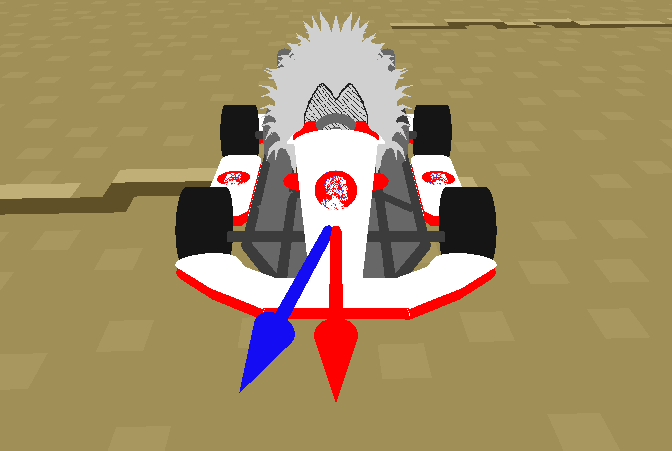
\includegraphics[width=0.8\textwidth]{figuras/direção.png}
    \caption{Seta de direção para o próximo ponto de destino.}
    \footnotesize{A figura mostra duas setas, uma em vermelho, cor do kart, que aponta com o ângulo do kart e outra em azul, que aponta para o ponto de destino do corredor, calculado por média ponderada por distância ponto a ponto do caminho mais curto.}
    \label{fig:arrow}
\end{figure}

\subsubsection{Modelo Elástico}

Para que o jogo fique dinâmico, foi implementado um modelo elástico, que é uma tática encontrado em jogos de corrida para que os corredores não tenham uma vantagem ou desvantagem muito grande, dessa forma, caso um corredor esteja muito atrás, ele terá uma velocidade maior, e caso um corredor esteja muito à frente, ele terá uma velocidade menor.

A cada iteração lógica do jogo temos um cálculo simples de diferença de 'pontuação' (proximidade do ponto de partida) entre o corredor e o jogador, e com isso é calculado uma velocidade adicional para o corredor, que é somada à velocidade atual, diminuindo a diferença entre os corredores.

Essa tática foi muito usada em jogos de corrida (veja em: \cite{rubberBandAi}) para que o jogo seja mais dinâmico e divertido, e foi implementado no USP Kart pelo mesmo motivo.